\documentclass[11pt]{article}
\usepackage[margin=2.5cm]{geometry}
\usepackage{booktabs}
\usepackage{float}
\usepackage{graphicx}
\usepackage{xcolor}
\usepackage{hyperref}
\title{GRouNdGAN Top-$k$ Causal-Graph Scaling Report}
\author{Auto-generated from \texttt{tf-k-experiment} run logs}
\date{\today}
\begin{document}\maketitle
\section{Overview}
This report analyses 15 completed runs in which the top-$k$ GRN parameter was varied from 1 to 15. The number of imposed edges is used as the independent variable throughout the scaling analysis. The HVG count, TF count, and target-gene count were intended to remain fixed.
\paragraph{Observed dimensions.} The logs show a small deviation from perfectly fixed dimensions: the $k=1$ run has 2,997 genes and 194 TFs, while most later runs have 3,000 genes and 197 TFs. The observed values are reported rather than silently normalised.
\section{GRN Characteristics}
\begin{table}[H]\centering
\caption{GRN statistics by top-$k$ setting. The independent variable is imposed-edge count.}
\begin{tabular}{rrrrrrrr}\toprule
Top-$k$ & TFs & Targets & Genes & TF/Target (\%) & Imposed Edges & Possible Edges & Density (\%) \\\midrule
1 & 194 & 2803 & 2997 & 6.92 & 2,803 & 543,782 & 0.5 \\
2 & 197 & 2803 & 3000 & 7.03 & 5,606 & 552,191 & 1.0 \\
3 & 197 & 2803 & 3000 & 7.03 & 8,409 & 552,191 & 1.5 \\
4 & 197 & 2803 & 3000 & 7.03 & 11,212 & 552,191 & 2.0 \\
5 & 197 & 2803 & 3000 & 7.03 & 14,015 & 552,191 & 2.5 \\
6 & 197 & 2803 & 3000 & 7.03 & 16,818 & 552,191 & 3.0 \\
7 & 197 & 2803 & 3000 & 7.03 & 19,621 & 552,191 & 3.6 \\
8 & 197 & 2803 & 3000 & 7.03 & 22,424 & 552,191 & 4.1 \\
9 & 197 & 2803 & 3000 & 7.03 & 25,227 & 552,191 & 4.6 \\
10 & 197 & 2803 & 3000 & 7.03 & 28,030 & 552,191 & 5.1 \\
11 & 197 & 2803 & 3000 & 7.03 & 30,833 & 552,191 & 5.6 \\
12 & 197 & 2803 & 3000 & 7.03 & 33,636 & 552,191 & 6.1 \\
13 & 197 & 2803 & 3000 & 7.03 & 36,439 & 552,191 & 6.6 \\
14 & 197 & 2803 & 3000 & 7.03 & 39,242 & 552,191 & 7.1 \\
15 & 197 & 2803 & 3000 & 7.03 & 42,045 & 552,191 & 7.6 \\
\bottomrule\end{tabular}\end{table}
\section{Training Step Times}
\begin{table}[H]\centering
\caption{Average final-step times for the controller and causal generator.}
\begin{tabular}{rrrr}\toprule Top-$k$ & Imposed Edges & Controller (ms) & Generator (ms) \\\midrule
1 & 2,803 & 42 & 71 \\
2 & 5,606 & 43 & 57 \\
3 & 8,409 & 41 & 60 \\
4 & 11,212 & 40 & 54 \\
5 & 14,015 & 39 & 71 \\
6 & 16,818 & 37 & 73 \\
7 & 19,621 & 38 & 101 \\
8 & 22,424 & 38 & 98 \\
9 & 25,227 & 41 & 126 \\
10 & 28,030 & 39 & 127 \\
11 & 30,833 & 41 & 159 \\
12 & 33,636 & 33 & 175 \\
13 & 36,439 & 40 & 185 \\
14 & 39,242 & 39 & 203 \\
15 & 42,045 & 38 & 228 \\
\bottomrule\end{tabular}\end{table}
\begin{table}[H]\centering
\caption{Expected duration for 200,000 controller steps and 500,000 generator steps.}
\begin{tabular}{rrrr}\toprule Top-$k$ & Imposed Edges & Controller & Generator / Total \\\midrule
1 & 2,803 & 2.3 h & 9.9 h / 12.2 h \\
2 & 5,606 & 2.4 h & 7.9 h / 10.3 h \\
3 & 8,409 & 2.3 h & 8.3 h / 10.6 h \\
4 & 11,212 & 2.2 h & 7.5 h / 9.7 h \\
5 & 14,015 & 2.2 h & 9.9 h / 12.0 h \\
6 & 16,818 & 2.1 h & 10.1 h / 12.2 h \\
7 & 19,621 & 2.1 h & 14.0 h / 16.1 h \\
8 & 22,424 & 2.1 h & 13.6 h / 15.7 h \\
9 & 25,227 & 2.3 h & 17.5 h / 19.8 h \\
10 & 28,030 & 2.2 h & 17.6 h / 19.8 h \\
11 & 30,833 & 2.3 h & 22.1 h / 24.4 h \\
12 & 33,636 & 1.8 h & 24.3 h / 26.1 h \\
13 & 36,439 & 2.2 h & 25.7 h / 27.9 h \\
14 & 39,242 & 2.2 h & 28.2 h / 30.4 h \\
15 & 42,045 & 2.1 h & 31.7 h / 33.8 h \\
\bottomrule\end{tabular}\end{table}
\section{Parameter Counts}
\begin{table}[H]\centering\resizebox{\textwidth}{!}{%
\begin{tabular}{rrrrrrrrrr}\toprule Top-$k$ & Edges & Generator & Critic & Labeler & Anti-Lab. & Gen. Opt. & Crit. Opt. & Labeler Opt. & Anti-Lab. Opt. \\\midrule
1 & 2,803 & 3.97M & 3.73M & 14.02M & 14.02M & 0.28M & 11.18M & 42.04M & 42.04M \\
2 & 5,606 & 4.15M & 3.73M & 14.03M & 14.03M & 0.49M & 11.19M & 42.05M & 42.05M \\
3 & 8,409 & 4.38M & 3.73M & 14.03M & 14.03M & 0.75M & 11.19M & 42.05M & 42.05M \\
4 & 11,212 & 4.66M & 3.73M & 14.03M & 14.03M & 1.06M & 11.19M & 42.05M & 42.05M \\
5 & 14,015 & 4.99M & 3.73M & 14.03M & 14.03M & 1.42M & 11.19M & 42.05M & 42.05M \\
6 & 16,818 & 5.36M & 3.73M & 14.03M & 14.03M & 1.83M & 11.19M & 42.05M & 42.05M \\
7 & 19,621 & 5.79M & 3.73M & 14.03M & 14.03M & 2.30M & 11.19M & 42.05M & 42.05M \\
8 & 22,424 & 6.27M & 3.73M & 14.03M & 14.03M & 2.81M & 11.19M & 42.05M & 42.05M \\
9 & 25,227 & 6.80M & 3.73M & 14.03M & 14.03M & 3.37M & 11.19M & 42.05M & 42.05M \\
10 & 28,030 & 7.38M & 3.73M & 14.03M & 14.03M & 3.99M & 11.19M & 42.05M & 42.05M \\
11 & 30,833 & 8.01M & 3.73M & 14.03M & 14.03M & 4.65M & 11.19M & 42.05M & 42.05M \\
12 & 33,636 & 8.69M & 3.73M & 14.03M & 14.03M & 5.36M & 11.19M & 42.05M & 42.05M \\
13 & 36,439 & 9.43M & 3.73M & 14.03M & 14.03M & 6.13M & 11.19M & 42.05M & 42.05M \\
14 & 39,242 & 10.21M & 3.73M & 14.03M & 14.03M & 6.95M & 11.19M & 42.05M & 42.05M \\
15 & 42,045 & 11.04M & 3.73M & 14.03M & 14.03M & 7.81M & 11.19M & 42.05M & 42.05M \\
\bottomrule\end{tabular}}\end{table}
\section{GPU Memory}
\begin{table}[H]\centering
\caption{Peak GPU memory by training phase.}
\begin{tabular}{rrrr}\toprule Top-$k$ & Imposed Edges & Controller (MiB) & Generator (MiB) \\\midrule
1 & 2,803 & 819 & 1,919 \\
2 & 5,606 & 795 & 2,113 \\
3 & 8,409 & 795 & 2,091 \\
4 & 11,212 & 1,309 & 2,897 \\
5 & 14,015 & 1,143 & 3,327 \\
6 & 16,818 & 795 & 3,699 \\
7 & 19,621 & 1,143 & 4,865 \\
8 & 22,424 & 1,309 & 5,971 \\
9 & 25,227 & 1,309 & 7,005 \\
10 & 28,030 & 795 & 7,643 \\
11 & 30,833 & 1,309 & 9,425 \\
12 & 33,636 & 1,309 & 10,799 \\
13 & 36,439 & 749 & 12,289 \\
14 & 39,242 & 1,143 & 13,703 \\
15 & 42,045 & 749 & 15,075 \\
\bottomrule\end{tabular}\end{table}
\section{Linear and Quadratic Fits}
Let $e$ denote the number of imposed edges. Ordinary least-squares fits over all completed runs give:
\begin{equation}
\widehat{M}_{\mathrm{gen}}(e) = 0.347271\,e - 932.5\ \mathrm{MiB},\qquad R^2=0.9504.
\end{equation}
\begin{equation}
\widehat{t}_{\mathrm{gen}}(e) = 0.004435\,e + 19.74\ \mathrm{ms/step},\qquad R^2=0.9173.
\end{equation}
\begin{equation}
\widehat{P}_{\mathrm{gen},2}(e) = 0.003207968\,e^2 + 36.156489\,e + 3848734.0\ \mathrm{parameters},\qquad R^2=1.0000.
\end{equation}
\begin{equation}
\widehat{M}_{\mathrm{gen},2}(e) = 0.000007201\,e^2 + 0.024320\,e + 1632.4\ \mathrm{MiB},\qquad R^2=0.9977.
\end{equation}
\begin{equation}
\widehat{t}_{\mathrm{gen},2}(e) = 0.000000109\,e^2 - 0.000437\,e + 58.44\ \mathrm{ms/step},\qquad R^2=0.9809.
\end{equation}
The quadratic fits substantially improve in-sample fit quality, but their extra curvature should be validated on additional top-$k$ values before extrapolation.
\section{Graphs}
\begin{figure}[H]\centering
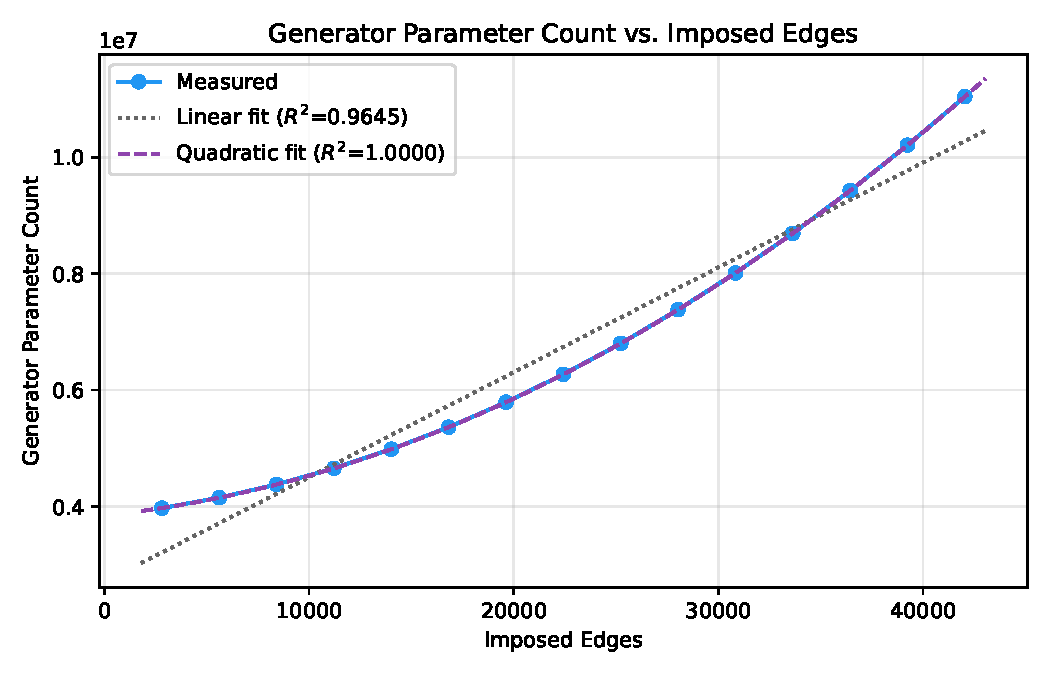
\includegraphics[width=0.95\textwidth]{gen_params_vs_edges.pdf}
\caption{Generator parameter count versus imposed edges.}\label{fig:params}
\end{figure}
\begin{figure}[H]\centering
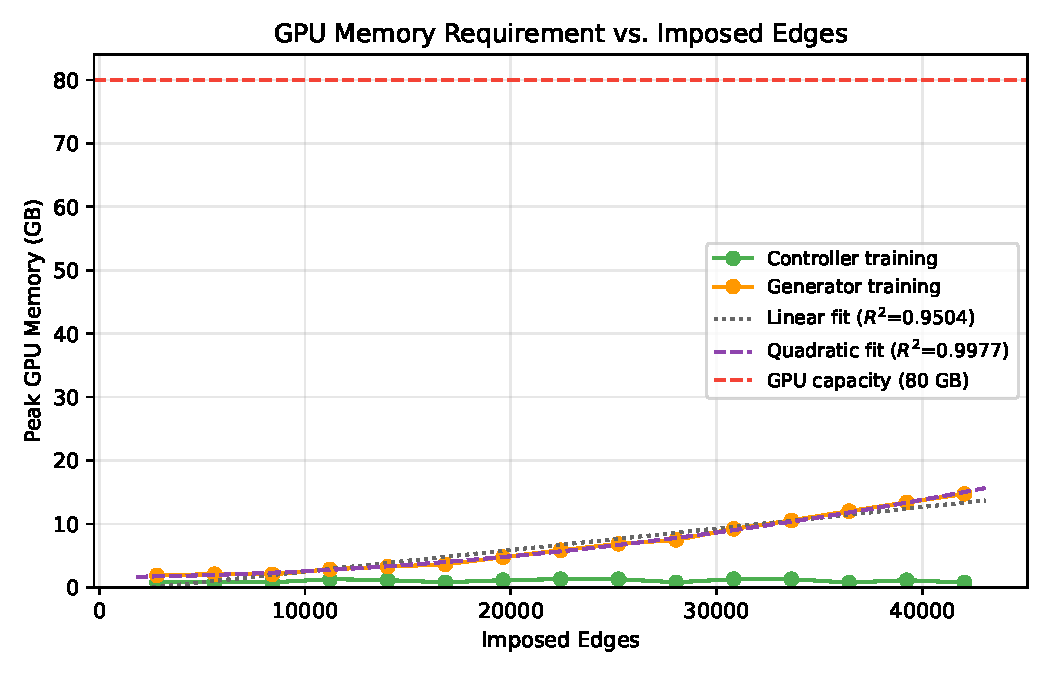
\includegraphics[width=0.95\textwidth]{gpu_mem_vs_edges.pdf}
\caption{Peak GPU memory versus imposed edges; the dashed line is the 80 GB GPU capacity.}\label{fig:memory}
\end{figure}
\begin{figure}[H]\centering
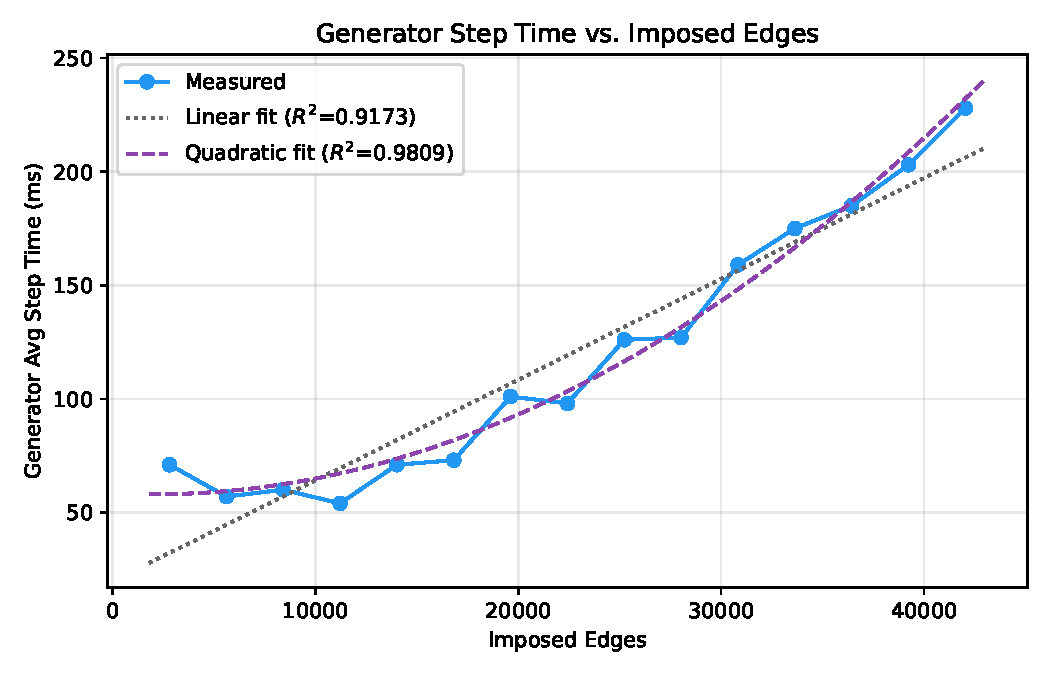
\includegraphics[width=0.95\textwidth]{gen_step_vs_edges.pdf}
\caption{Causal-generator average step time versus imposed edges.}\label{fig:time}
\end{figure}
\begin{figure}[H]\centering
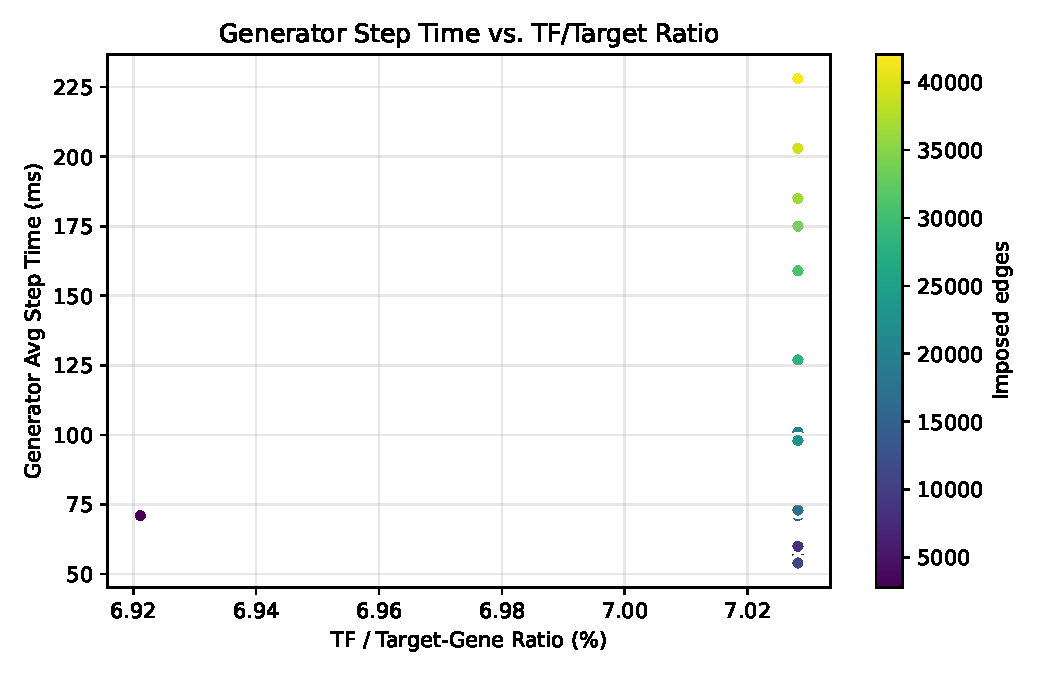
\includegraphics[width=0.95\textwidth]{gen_step_vs_ratio.pdf}
\caption{Causal-generator step time versus TF/target ratio; color indicates imposed-edge count.}\label{fig:ratio}
\end{figure}
\section{Notes}
\begin{itemize}
\item All included runs completed without CUDA out-of-memory errors.
\item Generator parameter count scales approximately linearly with imposed edges (linear $R^2=0.9645$; quadratic $R^2=1.0000$).
\item Quadratic fits improve the parameter-count $R^2$ from 0.9645 to 1.0000, the memory $R^2$ from 0.9504 to 0.9977, and the step-time $R^2$ from 0.9173 to 0.9809; this comparison is in-sample because all available top-$k$ values were used for fitting.
\item GPU memory is reported in MiB as measured by the monitoring CSV; the GPU capacity is 81,920 MiB.
\end{itemize}\end{document}